\chapter{Safety} 
\label{safety}
This chapter is about personnel safety, not equipment safety.  Learning to use HiFrost equipment properly without damaging anything is the aim this whole manual.  Safety of lab users, however, is important enough to warrant an entire devoted chapter, even if many points are reiterated throughout the document.

\vspace{1cm}
\fbox{\parbox{.93\textwidth}{\subsubsection{Ways to die or become seriously injured working on HiFrost:}
\begin{itemize}
\item Cryogenic explosions
\item Cryogenic burns
\item Oxygen depravation
\item Electric shock
\item Falling
\item Hot surfaces
\item Chemical exposure
\end{itemize}
}}

\section{Cryogenic Safety}
Both liquid nitrogen (\lnn, 77 K) and liquid helium (LHe, 4 K) are used during HiFrost operation.  The two primary cryogenic safety concerns are over-pressurization (explosion) of cryogenic vessels and cryogenic burns.  \lnn{} and LHe are each at risk of both, and precautions are taken while handling either. 
\subsection{Equipment}
\subsubsection{Cryogenic gloves}
Cryogenic gloves are lined internally with super-insulation and are long enough to cover past halfway between the wrist and elbow.  HiFrost equipment includes large and medium sized sets of gloves, and the best fitting size should always be used.  Typical activities requiring use of cryo gloves are filling the \lnn{} trap, inserting and removing LHe transfer lines, filling \lnn{} dewars for the target loading procedure, and making or manipulating target beads.

\subsubsection{Goggles}
Wearing googles and/or a face shield while handling open \lnn{} dewars is recommended.  Goggles also protect users in the vicinity of the large helium gas plumes expected during LHe dewar filling procedures.

\subsubsection{Closed toed shoes}
The general FEL safety regulations preclude anyone from wearing open toed shoes in controlled areas.  Still, there are areas outside the radiation perimeter where cryogens may be handled (e.g., the supply dewar just outside the bay doors), and closed toed shoes must be worn when handling \lnn{} or LHe vessels.
 
\subsection{Cryogenic Explosions}
The principle hazard of handling cryogens is an explosion caused by an enclosed volume of liquid warming up without adequate pressure relief for the evaporated gas.  For this reason, every container that holds cryogenic liquid has a pressure relief valve, and most large dewars have a non-configurable, one time use emergency burst disk.  


An important exception to the pressure relief rule is the \het{} circuit in the dilution refrigerator and pumping system.  Due to the scarcity and cost of \het, it is unacceptable to install pressure relief valves venting to atmosphere.  Instead, a single internal pressure relief valve, which opens at about 1.2 bar, is installed on the \het gas rack and should open if the pressure in the circuit rises due to a plug.  The pressure relief valve can only open if the valves leading to the fridge (via the condensor and still lines) are opened in the appropriate configuration.  Failure to do this could lead to catastrophic damage to the pumping system or, worse yet, the refrigerator itself.  

\subsubsection{Three valves rule}

The 500LD, 100LD and most supply helium dewars have three pathways for helium to escape in addition to the burst disk.  The three pathways are:
\begin{enumerate}
\item the pressurization port, where external gas is applied to the dewar
\item a pressure relief valve, usually set around 2-4 PSI
\item the inlet/outlet pathways where transfer lines connect through the top of the dewar 
\end{enumerate}

In general, all three of these ports may have manual valves to prevent helium from flowing through them.  For example, at the end of a 500LD fill, we close the outlet port on the filling dewar to halt the transfer, and the pressure relief valve is already closed to maintain liquid flow to the 500LD (see Section \ref{practical-op:500LDfill}).  The pressurization valve is always closed unless specifically venting the dewar or actively applying pressure to it.  The three valves rule is

\vsepfbox{\parbox{.93\textwidth}{\centering
\textbf{At least one of the three pathways on a cryogenic vessel must be open at all times.}
}}

If all three pathways are closed simultaneously, the radiative heat load (present in all dewars) will warm up the trapped liquid, increasing the pressure on the dewar until the burst disk breaks.  If for whatever reason the emergency burst disk fails, the resulting pressure will lead to an enormous explosion, easily fatal to any personnel nearby \cite{lnexplosion}. 

\subsection{Cryogenic Burns}
Cryogenic burns may happen by touching a liquid cryogen or cold gas plume, touching a bulk mass that was recently cooled by cryogenic liquid, or inhaling cold gas.  Use cryogenic gloves whenever handling liquid cryogens or surfaces they have recently cooled (like transfer lines), and always wear closed toed shoes in the lab.


\vspace{1cm}
\fbox{\parbox{.92\textwidth}{\subsubsection{In the event of a cryogenic burn\cite{epling}:}
\begin{itemize}
\item If prehospital warming is attempted, options include placing the affected area in warm (not hot) water or warming it using body heat (eg, placing frostbitten fingers in the axillae).
\item  You can flushing the area with tepid water but, in order to avoid tissue damage, a forceful flow of water should NOT be used.
\item Never use dry heat.  Never apply direct heat.
\item  Do not rewarm frostbitten tissue if there is a possibility of refreezing before reaching definitive care. This would result in worse tissue damage.
\item Do not rub frostbitten areas in an attempt to rewarm them; this can cause further tissue damage.
\item Remove any clothing or jewelry that may restrict circulation to injured area. 
\item  Do not cover the area; leave injured area open to air.
\end{itemize}
}}
\vspace{1cm}

To get help\cite{epling}, call Duke Employee Occupational Health and Wellness Hotline, available at any time, for assistance with a typical burn, 919-684-8115.  A Duke Hospital Operator with answer and then will page the EOHW nurse to your number.  During business hours you may also call EOHW main number, 919-681-3136, option 2 and ask for nurse.  Call 911 if situation is life threatening.  Provide the following information\cite{epling}:

\begin{itemize}
\item Agent causing cryogenic burn
\item Skin tone/color (white, pale, red, or blue).
\item Presence of Blisters (yes or no)
\item Location and area of injury
\item Presence of open skin (yes or no)
\item Current treatments
\item Any additional past medical information, medications, allergies
\item Confirm that the area of liquid nitrogen or hydrogen is secure and safe
\end{itemize}

\section{Oxygen Depravation}

Work with cryogenics automatically involves an oxygen depravation hazardous (ODH) environment, because the contents any liquid cryogen vessel are capable of displacing many times its volume of breathable air.  Generally, liquid helium can displace 1 cubic meter of breathing air for each liter of liquid that is quickly boiled, meaning the 100 L HiFrost dewar can displace 100 cubic meters of air.  Additionally, helium is colorless, odorless and tasteless, so it is often impossible for a worker to tell when they are not getting enough oxygen until the symptoms of oxygen deprivation begin to kick in.

The following information and the content of Table \ref{fig:jlabodh} is taken from Thomas Jefferson National Lab's ODH manual. \cite{jlabodh}

\paragraph{Health Effects of Reduced Oxygen}

Normal air is approximately 21\% oxygen and 78\% nitrogen. The remaining 1\% is mostly argon. Health effects begin at an oxygen concentration of 17\%. Oxygen monitors at Jefferson Lab are set to alarm at 19.5\%. This advance warning should give ample time to escape the hazard area.  The early health effects are difficult to detect so the oxygen monitors are relied upon to give early warning:

\begin{figure}
\centering
\begin{tabular}{|c|p{6cm}|}
 \hline
Percent Oxygen & Health Effects \\
\hline
17 & night vision reduced \newline increased breathing volume \newline accelerated heartbeat \\
\hline
16 & dizziness \newline reaction time for new tasks is doubled\\
\hline
15 & poor judgement \newline poor coordination \newline abnormal fatigue upon exertion \newline loss of muscle control\\
\hline
10-12 & very fault judgement \newline very poor muscular coordination \newline loss of consciousness\\
\hline
8-10& nausea \newline vomiting \newline coma\\
\hline
$<$8 & Permanent brain damage \\
\hline
$<$6 & spasmodic breathing \newline convulsive movements \newline death in 5-8 minutes \\
\hline
\end{tabular} 
\caption{JLab ODH manual's list of health effects of oxygen deprivation.}
\label{fig:jlabodh}
\end{figure}

\section{High Voltage Safety}

The EIO power supply (Cober) outputs a maximum 10 kV, 100 mA power across HVlines from the pump station area to the GV.  The only interlock on the power supply is on the door that opens the back panel, which immediately turns off all HV.

\begin{figure}[htbp!]
 \centering
 \begin{minipage}{0.45\textwidth}
   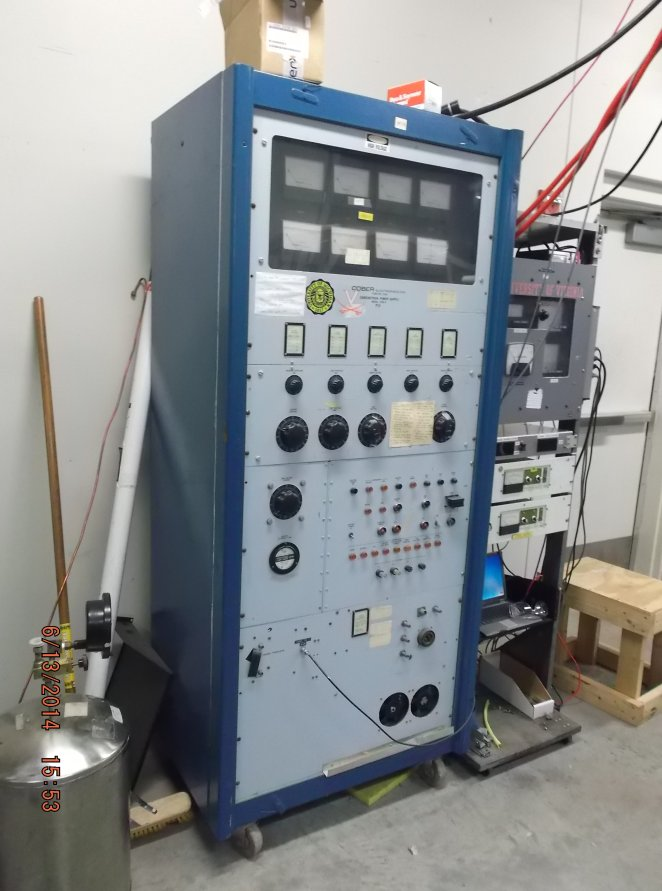
\includegraphics[width=\textwidth]{./img/hv-safety-racks.jpg}
   \caption{EIO power supply (Cober) and breakout panel rack.}
 \label{fig:hv-safety-racks}
  \end{minipage}
 \quad
  \begin{minipage}{0.45\textwidth}
   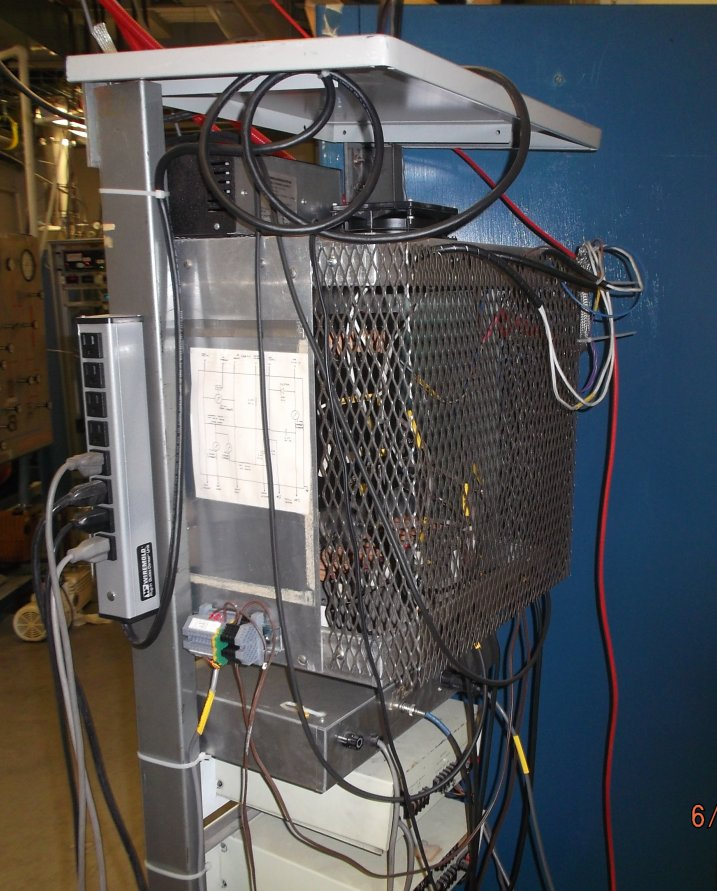
\includegraphics[width=\textwidth]{./img/hv-safety-cage.jpg}
   \caption{Protective cage around EIO breakout panel (rear).}
 \label{fig:hv-safety-cage}
  \end{minipage}
\end{figure}


The cage-protected back of the power supply breakout rack is also a risk to personnel, but there is no interlock to kill the HV when the cage is opened.  Nothing should be reached inside the cage, and the cage should not be removed, while the power supply is active.

In the GV, the HV wires are enclosed in a plastic red sheath for insulation and visibility.  They connect to a breakout panel behind the EIO, which is protected by a transparent plastic cover.  There is no interlock on this cover, so it should never be removed while the power supply is active.

The EIO itself is not at HV, and is not an electrical hazard to personnel.  However, it is very delicate and should not be worked on with ferromagnetic tools (see magnet safety section below).
\begin{figure}[htbp!]
 \centering
 \begin{minipage}{0.45\textwidth}
   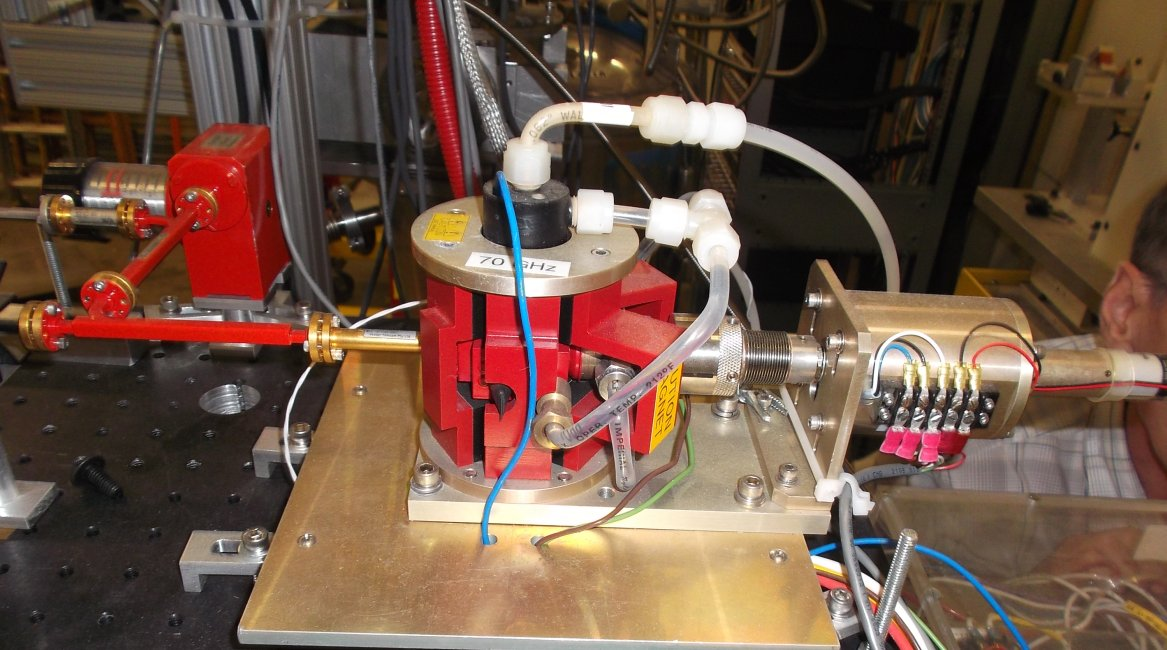
\includegraphics[width=\textwidth]{./img/hv-safety-eio.jpg}
   \caption{The EIO.}
 \label{fig:hv-safety-eio}
  \end{minipage}
 \quad
  \begin{minipage}{0.45\textwidth}
   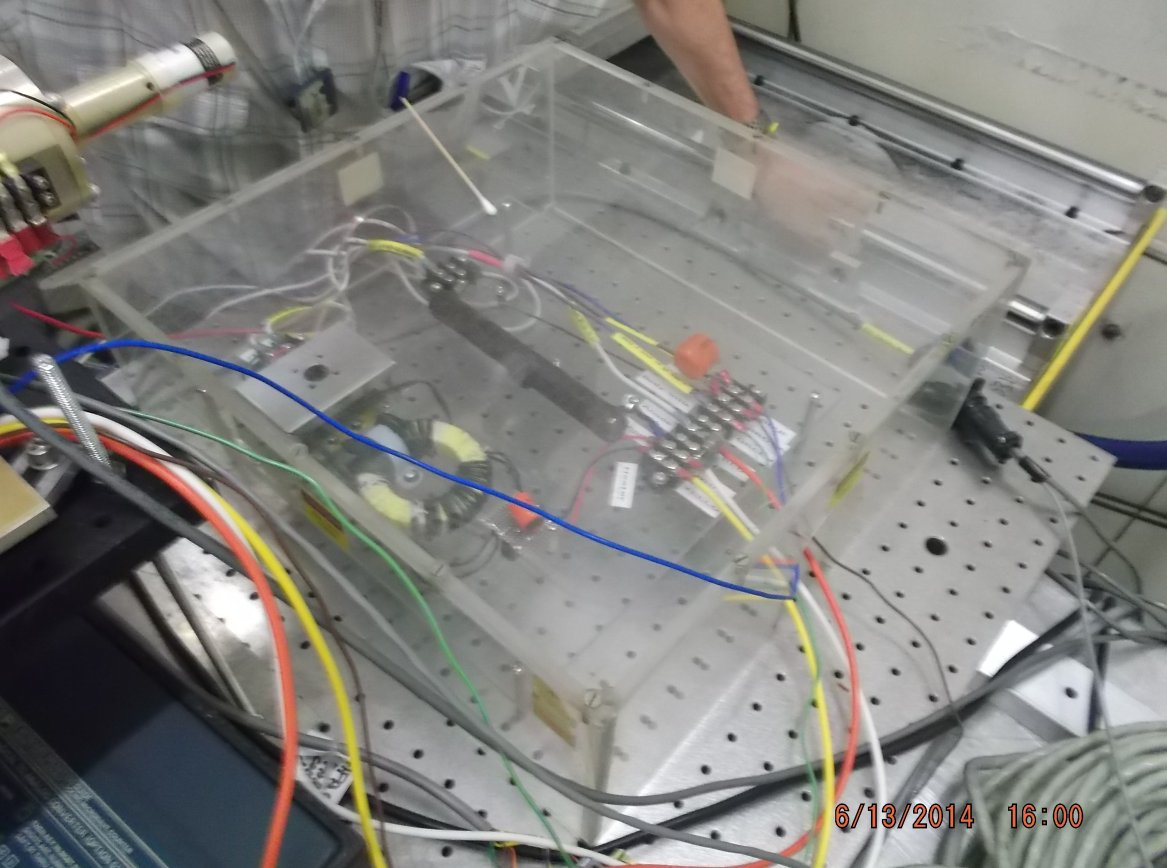
\includegraphics[width=\textwidth]{./img/hv-safety-eio-breakout.jpg}
   \caption{The breakout box located behind the EIO in the GV.}
 \label{fig:hv-safety-eio-breakout}
  \end{minipage}
\end{figure}
\section{Gravity Safety}

No high places should be reached without the appropriate ladder during Hifrost operations or activities.  Remember the following 5 rules of ladder safety\cite{laddersafety-duke}:
\begin{enumerate}
 \item Choose the right ladder for the job.
 \item Inspect the ladder before you use it.
 \item Set up the ladder with care.
 \item Climb and descend ladders cautiously.
 \item Use safe practices when working on a ladder.
\end{enumerate}

Additional information ladder safety is provided by OSHA\cite{laddersafety-osha}.

\section{Magnetic Field Safety}

Aside from being full of 77 K liquid nitrogen and 4 K liquid helium, the polarizing magnet poses a safety threat by virtue of its 2.5 T field.  The 0.5 T frozen spin field is considerably weaker and, due to its localization inside the radiation shield of the fridge, less accessible to personnel and foreign objects.

The most likely danger is a ferromagnetic object (like a wrench) striking personnel as it is pulled towards the polarizing magnet\cite{magnetsafety}.  The best safety measure against this is making sure Hifrost workers and anyone else in the GV know when the magnet is on and do not keep loose ferromagnetic objects on their person.

Anyone with an implanted medical device, such as a pacemaker, should alert Hifrost officials before working on or near Hifrost equipment during a polarizing magnet cooldown.  Under no circumstances should they get closer than the 10 gauss line while the magnet is energized without speaking with their physician and the director of DFELL\cite{pacemakersafety}.

The EIO has a strong enough magnetic field to pull a ferromagnetic object in from a few inches away, so care should be taken to not allow any loose tools to smash into it.

\section{Chemical Safety}
\subsection{Heavy elements}
\subsubsection{Indium}
Indium is used for sealing two interfacing sets of flanges in the dilution refrigerator.  Disassembling the refrigerator necessarily entails scraping indium off these flanges, and assembling the fridge requires cutting and setting the seal from a roll of indium wire.

While no cases of indium poisoning by oral consumption have been recorded, it remains a heavy element and toxic to humans if it enters the blood stream.  As a precaution, wearing latex gloves is recommended while handling indium, and hands should be washed immediately after, especially before taking a lunch break or leaving for the day.

\subsubsection{Lead}
Lead is a toxic metal often used in the laboratory due to its density and availability.  Inorganic lead is not readily absorbed through the skin, but once it enters the body (through ingestion or inhalation) it is carried by the bloodstream to the ``bone, teeth, liver, lungs, kidneys, brain and spleen'' in high concentrations \cite{aafp98}.  Children and pregnant women are particularly at risk to damage from lead poisoning \cite{epa13}


Lead bricks are used at the University of Virginia PTGroup lab to counter the weight of the fridge on the stand.  Lead bricks are also present at HIGS around the beam line and UTR, although they are not usually found in the Vault.  Work gloves and hard-toed shoes are recommended when carrying or lifting lead bricks.  Any skin that was exposed to lead bricks or lead dust should be washed immediately after performing duties requiring lead exposure.

\subsection{Isopropyl Alcohol}
Isopropyl alcohol is used to clean the indium and KF-oring surfaces on the fridge and in the pumping system.  It is generally safe to be exposed to, but if there is a large quantity in an open container (like a bath for soaking vacuum parts) make sure the area is well ventilated and anyone working nearby knows about it.  Symptoms of isopropyl alcohol inhalation are dizziness, drowsiness and headache, and may cause unconsciousness \cite{isopropmsds}. 

Isopropyl alcohol has a flash point (the lowest temperature it emits ignitable fumes) of 53$^\circ$ F, and care should be taken not to expose alcohol bottles to open flames.